\documentclass[dvipsnames, aspectratio=169]{beamer}
\usepackage[utf8]{inputenc}
\usepackage{listings}
\usepackage{comment}
\usepackage{soul}
%\usepackage{ulem}
\usepackage{subfig}
\usepackage{pgf-pie}
\setul{}{1pt}
\usepackage[oldenum, olditem]{paralist}
%allow even smaller text
\newcommand\tinytiny{\fontsize{4pt}{3}\selectfont}

\makeatletter
\let\old@lstKV@SwitchCases\lstKV@SwitchCases
\def\lstKV@SwitchCases#1#2#3{}
\makeatother
\usepackage{lstlinebgrd}
\makeatletter
\let\lstKV@SwitchCases\old@lstKV@SwitchCases

\lst@Key{numbers}{none}{%
    \def\lst@PlaceNumber{\lst@linebgrd}%
    \lstKV@SwitchCases{#1}%
    {none:\\%
     left:\def\lst@PlaceNumber{\llap{\normalfont
                \lst@numberstyle{\thelstnumber}\kern\lst@numbersep}\lst@linebgrd}\\%
     right:\def\lst@PlaceNumber{\rlap{\normalfont
                \kern\linewidth \kern\lst@numbersep
                \lst@numberstyle{\thelstnumber}}\lst@linebgrd}%
    }{\PackageError{Listings}{Numbers #1 unknown}\@ehc}}
\makeatother


\usepackage{tikz}
\graphicspath{{4_5/figures/}}

%disclaimer for Sandia. uncomment and the whole blob goes away @ b80c116300122
%\def\sandid{SANDXXXX PE}

% \title{Performance Portability with Kokkos}
\title{Kokkos 4.5 Release Briefing}

%BAD misuse of author field
\author{New Capabilities}

\date{2024-12-10}

\usetheme{kokkos}

\newif\ifshort
\newif\ifmedium
\newif\iffull
\newif\ifnotoverview

\newcommand{\TutorialDirectory}{\texttt{Intro-Full}}
\newcommand{\ExerciseDirectory}[1]{\texttt{Exercises/#1/}}
\newcommand{\TutorialClone}{\texttt{Kokkos/kokkos-tutorials/\TutorialDirectory}}

\definecolor{darkgreen}{rgb}{0.0, 0.5, 0.0}
\definecolor{darkred}{rgb}{0.8, 0.0, 0.0}
\definecolor{orange}{rgb}{0.8, 0.33, 0.0}
\definecolor{purple}{rgb}{0.60, 0.20, 0.80}
\colorlet{bodyColor}{blue!20}
\colorlet{patternColor}{orange!30}
\colorlet{policyColor}{green!30}

% http://tex.stackexchange.com/questions/144448/color-a-text-line-in-a-code-lstlisting
\lstnewenvironment{code}[1][]%
{
  %with txfonts: OT1/txr/m/n/10
  %with default fonts: OT1/cmr/m/n/10
  %\fontfamily{cmr}\selectfont
  %\showthe\font
   \noindent
   \minipage{\linewidth}
   %\vspace{0.5\baselineskip}
   \lstset{mathescape, escapeinside={<@}{@>},
moredelim=**[is][{\btHL[fill=patternColor]}]{@pattern}{@pattern},
moredelim=**[is][{\btHL[fill=red!30]}]{@warning}{@warning},
moredelim=**[is][{\btHL[fill=policyColor]}]{@policy}{@policy},
moredelim=**[is][{\btHL[fill=bodyColor]}]{@body}{@body},
moredelim=**[is][{\btHL[fill=red!30]}]{@warning}{@warning},
moredelim=**[is][\color{black}]{@black}{@black},
moredelim=**[is][\color{blue}]{@blue}{@blue},
moredelim=**[is][\bf]{@bold}{@bold},
moredelim=**[is][\it]{@italic}{@italic},
moredelim=**[is][\color{boldblue}\bf]{@boldblue}{@boldblue},
moredelim=**[is][\color{red}]{@red}{@red},
moredelim=**[is][\color{green}]{@green}{@green},
moredelim=**[is][\color{gray}]{@gray}{@gray},
moredelim=**[is][\color{darkgreen}]{@darkgreen}{@darkgreen},
moredelim=**[is][\color{darkred}]{@darkred}{@darkred},
moredelim=**[is][\color{orange}]{@orange}{@orange},
moredelim=**[is][\color{purple}]{@purple}{@purple},
keywords={},
#1}
}
{
  \endminipage
  %\vspace{1.0\baselineskip}
}

\makeatletter
\newif\ifATOlinebackground
\lst@Key{linebackground}{\tiny}{\def\ATOlinebackground{#1}\global\ATOlinebackgroundtrue}
\makeatother

\lstnewenvironment{shell}[1][]{%
  \global\ATOlinebackgroundfalse
  \lstset{language=sh,%
    showstringspaces=false,
    aboveskip=0pt,
    frame=none,
    numbers=none,
    belowskip=2pt,
    breaklines=true,
    #1,
    }
  %\ifATOlinebackground
  \lstset{linebackgroundcolor={
    \ATOlinebackground
  }}
  %\fi
  }{}

\lstnewenvironment{cmake}[1][]{%
  \global\ATOlinebackgroundfalse
  \lstset{language=sh,%
    showstringspaces=false,
    aboveskip=0pt,
    frame=none,
    numbers=none,
    belowskip=2pt,
    breaklines=true,
    #1,
    }
  %\ifATOlinebackground
  \lstset{linebackgroundcolor={
    \ATOlinebackground
  }}
  %\fi
  }{}

\newcommand{\inlinecode}[1]{{\lstset{basicstyle=\ttfamily,keywordstyle={},showstringspaces=false}\lstinline$#1$}}
\newcommand{\inlineshell}[1]{{\lstset{basicstyle=\ttfamily,keywordstyle={},showstringspaces=false}\lstinline$#1$}}

\setbeamercolor{block title}{fg=white, bg=SandiaLightBlue}
\setbeamercolor{block body}{bg=lightgray}
\setbeamercolor{block title alerted}{fg=white, bg=SandiaRed}
\setbeamercolor{block body alerted}{bg=lightgray}



%\usepackage[texcoord,grid,gridunit=mm,gridcolor=red!10,subgridcolor=green!10]{eso-pic}
\usepackage[absolute,overlay]{textpos}





% http://tex.stackexchange.com/questions/8851/how-can-i-highlight-some-lines-from-source-code

\usepackage{pgf, pgffor}
\usepackage{listings}
\usepackage{lstlinebgrd} % see http://www.ctan.org/pkg/lstaddons

\makeatletter
%%%%%%%%%%%%%%%%%%%%%%%%%%%%%%%%%%%%%%%%%%%%%%%%%%%%%%%%%%%%%%%%%%%%%%%%%%%%%%
%
% \btIfInRange{number}{range list}{TRUE}{FALSE}
%
% Test in int number <number> is element of a (comma separated) list of ranges
% (such as: {1,3-5,7,10-12,14}) and processes <TRUE> or <FALSE> respectively

\newcount\bt@rangea
\newcount\bt@rangeb

\newcommand\btIfInRange[2]{%
    \global\let\bt@inrange\@secondoftwo%
    \edef\bt@rangelist{#2}%
    \foreach \range in \bt@rangelist {%
        \afterassignment\bt@getrangeb%
        \bt@rangea=0\range\relax%
        \pgfmathtruncatemacro\result{ ( #1 >= \bt@rangea) && (#1 <= \bt@rangeb) }%
        \ifnum\result=1\relax%
            \breakforeach%
            \global\let\bt@inrange\@firstoftwo%
        \fi%
    }%
    \bt@inrange%
}
\newcommand\bt@getrangeb{%
    \@ifnextchar\relax%
        {\bt@rangeb=\bt@rangea}%
        {\@getrangeb}%
}
\def\@getrangeb-#1\relax{%
    \ifx\relax#1\relax%
        \bt@rangeb=100000%   \maxdimen is too large for pgfmath
    \else%
        \bt@rangeb=#1\relax%
    \fi%
}

%%%%%%%%%%%%%%%%%%%%%%%%%%%%%%%%%%%%%%%%%%%%%%%%%%%%%%%%%%%%%%%%%%%%%%%%%%%%%%
%
% \btLstHL<overlay spec>{range list}
%
% TODO BUG: \btLstHL commands can not yet be accumulated if more than one overlay spec match.
%
\newcommand<>{\btLstHL}[2]{%
  \only#3{\btIfInRange{\value{lstnumber}}{#1}{\color{#2}\def\lst@linebgrdcmd{\color@block}}{\def\lst@linebgrdcmd####1####2####3{}}}%
}%
\makeatother






% http://tex.stackexchange.com/questions/15237/highlight-text-in-code-listing-while-also-keeping-syntax-highlighting
%\usepackage[T1]{fontenc}
%\usepackage{listings,xcolor,beramono}
\usepackage{tikz}

\makeatletter
\newenvironment{btHighlight}[1][]
{\begingroup\tikzset{bt@Highlight@par/.style={#1}}\begin{lrbox}{\@tempboxa}}
{\end{lrbox}\bt@HL@box[bt@Highlight@par]{\@tempboxa}\endgroup}

\newcommand\btHL[1][]{%
  \begin{btHighlight}[#1]\bgroup\aftergroup\bt@HL@endenv%
}
\def\bt@HL@endenv{%
  \end{btHighlight}%
  \egroup
}
\newcommand{\bt@HL@box}[2][]{%
  \tikz[#1]{%
    \pgfpathrectangle{\pgfpoint{1pt}{0pt}}{\pgfpoint{\wd #2}{\ht #2}}%
    \pgfusepath{use as bounding box}%
    \node[anchor=base west, fill=orange!30,outer sep=0pt,inner xsep=1pt, inner ysep=0pt, rounded corners=3pt, minimum height=\ht\strutbox+1pt,#1]{\raisebox{1pt}{\strut}\strut\usebox{#2}};
  }%
}
\makeatother



\usetikzlibrary{calc}
\usepackage{xparse}%  For \NewDocumentCommand

% tikzmark command, for shading over items
\newcommand{\tikzmark}[1]{\tikz[overlay,remember picture] \node (#1) {};}

\makeatletter
\NewDocumentCommand{\DrawBox}{s O{}}{%
    \tikz[overlay,remember picture]{
    \IfBooleanTF{#1}{%
        \coordinate (RightPoint) at ($(left |- right)+(\linewidth-\labelsep-\labelwidth,0.0)$);
    }{%
        \coordinate (RightPoint) at (right.east);
    }%
    \draw[red,#2]
      ($(left)+(-0.2em,0.9em)$) rectangle
      ($(RightPoint)+(0.2em,-0.3em)$);}
}

\NewDocumentCommand{\DrawBoxWide}{s O{}}{%
    \tikz[overlay,remember picture]{
    \IfBooleanTF{#1}{%
        \coordinate (RightPoint) at ($(left |- right)+(\linewidth-\labelsep-\labelwidth,0.0)$);
    }{%
        \coordinate (RightPoint) at (right.east);
    }%
    \draw[red,#2]
      ($(left)+(-\labelwidth,0.9em)$) rectangle
      ($(RightPoint)+(0.2em,-0.3em)$);}
}

\NewDocumentCommand{\DrawBoxWideBlack}{s O{}}{%
    \tikz[overlay,remember picture]{
    \IfBooleanTF{#1}{%
        \coordinate (RightPoint) at ($(left |- right)+(\linewidth-\labelsep-\labelwidth,0.0)$);
    }{%
        \coordinate (RightPoint) at (right.east);
    }%
    \draw[black,#2]
      ($(left)+(-\labelwidth,0.9em)$) rectangle
      ($(RightPoint)+(0.2em,-0.3em)$);}
}
\makeatother

\usetikzlibrary{positioning}

\usetikzlibrary{shapes}

\hypersetup{
    colorlinks=true,
    linkcolor=blue,
    filecolor=magenta,
    urlcolor=cyan,
}



\shorttrue
\mediumfalse
\fullfalse

\begin{document}

\begin{frame}
  \titlepage
\end{frame}


\begin{frame}[fragile]{Outline}

  \textbf{4.5 Release Highlights}

  \begin{itemize}
    \item{Organizational}
    \item{SequentialHostInit}
    \item{Feature Highlights}
    \item{General Enhancements}
    \item{Graphs Enhancements}
    \item{Backend updates}
    \item{Tuning changes demo}
    \item{Build system updates}
    \item{Deprecations and other breaking changes}
    \item{Bug Fixes}
  \end{itemize}

\end{frame}

\begin{frame}{Find More}

  \textbf{Online Resources}:

  \begin{itemize}
    \item \url{https://github.com/kokkos}:
          \begin{itemize}
            \item Primary Kokkos GitHub Organization
          \end{itemize}
    \item \url{https://github.com/kokkos/kokkos-tutorials/wiki/Kokkos-Lecture-Series}:
          \begin{itemize}
            \item{Slides, recording and Q\&A for the Full Lectures}
          \end{itemize}
    \item \url{https://kokkos.org/kokkos-core-wiki}:
          \begin{itemize}
            \item Wiki including API reference
          \end{itemize}
    \item \url{https://kokkosteam.slack.com}:
          \begin{itemize}
            \item Slack workspace for Kokkos.
            \item Please join: fastest way to get your questions answered.
            \item Can whitelist domains, or invite individual people.
          \end{itemize}
  \end{itemize}

\end{frame}

\begin{frame}[fragile]{Kokkos Usage}
  \textbf{Would like to strengthen community bonds and discoverability}

  \vspace{10pt}
  \textit{List of Applications and Libraries}
  \begin{itemize}
    \item Add your app to \url{https://github.com/kokkos/kokkos/issues/1950}
    \item We are planning to add that to a Kokkos website.
    \item Helps people discover each other when working on similar things.
  \end{itemize}

  \vspace{10pt}
  \textit{GitHub Topics}
  \begin{itemize}
    \item Use \textit{kokkos} tag on your repos.
    \item If you click on the topic you get a list of all projects on github with that topic.
  \end{itemize}
\end{frame}


%==========================================================================

\begin{frame}[fragile]

  {\Huge Organizational}

  \vspace{10pt}

  \textbf{Content:}
  \begin{itemize}
    \item HPSF and Kokkos Meeting 2025
    \item Targetting C++20 for Kokkos 5.0
    \item SequentialHostInit and Views of Views 
  \end{itemize}

\end{frame}

%==========================================================================

\begin{frame}[fragile]{Kokkos User Group Meeting 2025}
\begin{center}
\textbf{Kokkos User Group Meeting 2025 @ HPSF Conference}
\end{center}

\begin{itemize}
\item{\textit{When:} May 5th-8th 2025}
\item{\textit{Where:} Chicago}
\item{\textit{What:} 2-days HPSF plenary + 2-days Project meetings}
\item{\textit{KUG-Content Request:} Focused on user experiences
\begin{itemize}
   \item{How do you leverage Kokkos?}
   \item{What are pain points?}
   \item{Kokkos based libraries of interest for the community}
\end{itemize}
}
\end{itemize}


\vspace{10pt}

\begin{center}
\textit{Registration will open in January!}
\end{center}
\end{frame}


\begin{frame}[fragile]{Kokkos 5 and ISO C++20}
\begin{center}
\textbf{Kokkos 5 is comming Summer 2025}

\vspace{0.5cm}
\textbf{We will require C++20!}
\end{center}

\textit{Start preparing now:}
\begin{itemize}
  \item{Check availability of compilers on your systems}
  \item{Test with C++20 enabled: start with a CPU build}
  \item{Minimum Compiler requirements will change (more details later)}
\end{itemize}

\vspace{0.5cm}
\begin{center}
\textit{Nothing wrong for your project to require C++20 now if you feel ready!}
\end{center}
\end{frame}


%==========================================================================

\begin{frame}[fragile]

  {\Huge View of Views}
  
    \vspace{10pt}

\end{frame}

%==========================================================================

\begin{frame}[fragile]{End of view object lifetime}

What happens when a view object gets out of scope?
\begin{code}
{
  View<T*, HostSpace> v("v", n);
  // [...]
}  // calls view destructor, i.e. v.~View()
\end{code}

\pause
\begin{code}
   // equivalent to:
   //   parallel_for(
   //     RangePolicy<DefaultHostExecutionSpace>(0, n),
   //     KOKKOS_LAMBDA(size_t i) { v(i).~T(); }
   //   );
   //   kokkos_free(v.data());
\end{code}

\pause
\bigskip
Now, what if \texttt{T} is a view, or some user-defined type that contains a view?

\end{frame}

%==========================================================================

\begin{frame}[fragile]{The infamous View of Views}

Our programming guide states it clearly (paraphrased):

\begin{quote}
Please don't. \\
But, if you do, here is the right way to do it:
\end{quote}

\pause
\begin{code}
using Naughty = Kokkos::View<T*, SomeMemorySpace>
View<Naughty**, HostSpace> v(view_alloc("v", WithoutInitializing), 2, 3);
// create and initiliaze elements with a placement new
new &v(0,0) Naughty("w00", 4);
new &v(1,0) Naughty("w10", 5);
new &v(0,1) Naughty("w01", 6);
// [...]
// must **manually** call the elements destructor
v(0,0).~Naughty();
v(1,0).~Naughty();
v(0,1).~Naughty();
\end{code}

Lifetime management of element objects is the user's responsability, and it must be done on the host, \textbf{not with a parallel region}.

\end{frame}

%==========================================================================

\begin{frame}[fragile]{What if I forgot to clean up?}

\begin{columns}
\begin{column}{0.65\textwidth}
    What happens depends on how the (outter) view was constructed:
    \begin{itemize}
    \item If you passed the \texttt{WithoutInitializing} allocation property, you potentially leak resources
    \item Otherwise, you program may hang when you upgrade to 4.4
        \begin{itemize}
        \item Outter view destructor launches a parallel region to end the lifetime of individual elements
        \item If an individual element being destructed causes some non-empty (inner) view to go out of scope, Kokkos semantics are being violated
        \item Inner view object being destroyed leads to an attempt to acquire the lock that is already engaged for the outter view cleanup
        \end{itemize}
    \end{itemize}
\end{column}
\begin{column}{0.35\textwidth}
    \begin{center}
    
\includegraphics[width=\linewidth]{4_4/cleanupafteryourself}
    \end{center}
\end{column}
\end{columns}

\end{frame}

%==========================================================================

\begin{frame}[fragile]{New SequentialHostInit view allocation property in 4.5}

\begin{itemize}
\item Introduced new \texttt{SequentialHostInit} view allocation property in \texttt{develop}
\item Does not support non-default-constructible element types
\item May backport it to a 4.4.1 patch release if there is strong appetite for it
\end{itemize}

\begin{code}
using Naughty = Kokkos::View<T*, SomeMemorySpace>
View<Naughty**, HostSpace> v(view_alloc("v", SequentialHostInit), 2, 3);
// copy assign elements
v(0,0) = Naughty("w00", 4);
v(1,0) = Naughty("w10", 5);
v(0,1) = Naughty("w01", 6);
// v.~View() handles properly elements destruction
\end{code}

\end{frame}


%==========================================================================

\begin{frame}[fragile]

  {\Huge Feature highlights}

  \vspace{10pt}

\end{frame}

\begin{frame}[fragile]{MDSpan-based View Implementation}
  % what
  \begin{itemize}
    \item This release contains an extensive refactoring of \texttt{Kokkos::View}
    \item View was refactored to use the \texttt{mdspan}, a C++23 addition to the standard library
    \begin{itemize}
      \item \texttt{mdspan} is backported to C++17/C++20, and our implementation can be found at \url{github.com/kokkos/mdspan/}
    \end{itemize}
    \item The goal of this refactor was to provide better library interoperability, more API flexibility, and reduced maintenance burden
    \item In principle, this update should be fully transparent; i.e. your existing code should work as it did before and we've done extensive testing to ensure this
    \end{itemize}
% motivation
% example
% What does this mean for apps
\end{frame}

%==========================================================================

\begin{frame}[fragile]{MDSpan-based View Implementation}
  \begin{itemize}
  \item What does this mean for applications?
  \begin{itemize}
    \item We use the same customization points as mdspan now, including accessors and layout mappings
    \item This is also how we are working on support for Sacado with the new view implementation
    \begin{itemize}
      \item We don't have to special-case as much for Sacado inside of Kokkos anymore
      \item Full Sacado support coming in patch release
    \end{itemize}
    \item In the future, we may provide a mechanism for users to customize these. Would that be useful for people?
  \end{itemize}
  \end{itemize}
\end{frame}

%==========================================================================


\begin{frame}[fragile]{Updates on Kokkos Graphs}
 \begin{itemize}
     \item Reminder: \emph{Kokkos Graph} is an abstraction of computation represented as a DAG
     \item Located in~\emph{Kokkos::Experimental}
      \item Example of a diamond-shaped compute graph supported
      \begin{code}[keywords={std}]
      auto graph = Kokkos::create_graph([&](auto root) {
      auto nodeA = root.then_parallel_for("workloadA",policy,functor);
      auto nodeB = nodeA.then_parallel_for("workloadB",policy,functor);
      auto nodeC = nodeA.then_parallel_for("workloadC",policy,functor);
      auto nodeD = Kokkos::when_all(nodeB, nodeC).
        then_parallel_for("workloadD",policy,functor);});
      graph.instantiate();
      graph.submit();
      \end{code}
     \item Supports Kokkos patterns (\texttt{then\_parallel\_*}, \texttt{then})
     \item We have two new features to support more use-cases (subgraphs via stream-capture and host-nodes)
 \end{itemize}
\end{frame}

%==========================================================================


\begin{frame}[fragile]{Updates on Kokkos Graphs (Capture)}
 \begin{itemize}
     \item Adds support for subgraphs created using stream-capture via \texttt{*\_capture(...)}
     \begin{itemize}      
      \item Useful to include native code and libraries
      \item Calls internally \texttt{*StreamBeginCapture},\texttt{*StreamEndCapture}
    \end{itemize}
     \item Example: Using cuBLAS
        \begin{code}[keywords={std}]
    auto graph = Kokkos::Experimental::create_graph([&](const auto& root){
      auto handle = create_cublas_handle();
       /* NEW! */
      root.cuda_capture(exec,
      [=](const Kokkos::Cuda& exec_){
        /* Body of lambda using CUDA */
        cublasSetStream(handle.get(),exec_.cuda_stream()));
        cublasDgemv( handle.get(),CUBLAS_OP_N,...);
      });
    });
    graph.instantiate(); 
    graph.submit(exec);
      \end{code}
    \item Supported backends: HIP, CUDA, SYCL (\emph{*\_capture})
 \end{itemize}
\end{frame}

%==========================================================================

\begin{frame}[fragile]{Updates on Kokkos Graphs (then\_host)}
 \begin{itemize}
     \item Adds support for host-side graph nodes    
    \begin{itemize}
      \item New API: \texttt{then\_host(...)}
      \item Calls internally \texttt{*GraphAddHostNode}
    \end{itemize}
 \item Example: Using a host-side graph node
        \begin{code}[keywords={std}]
    ...
    template<>
    class functor<Kokkos::DefaultExecutionSpace>{ /* Device code */ };
    template<>
    class functor<Kokkos::HostSpace> { /* Host code*/ };
    auto graph = Kokkos::Experimental::create_graph(exec, 
        [&](const auto& root) {
          root.then ("NodeA",exec,functor<Kokkos::DefaultExecutionSpace>{})
          /* NEW! */
          .then_host("NodeB",functor<Kokkos::HostSpace>{});
    });      
      \end{code}
  
  \item We explicitly use an execution policy with Kokkos::LaunchBounds$\langle 1\rangle$ to execute a \emph{then} graph node
 \end{itemize}
\end{frame}


%==========================================================================

\begin{frame}[fragile]{Updates on Kokkos Graphs (then\_host)}
 \begin{itemize}
 \item Example: Using a host-side graph node (continued)
        \begin{code}[keywords={std}]
    using view_t = View<int*,Kokkos::MemoryTraits<Unmanaged>>
    view_t v;
    ...
    template<>
    class functor<HostSpace> {
      view_t v;
      void operator()() const { v = view_t(Kokkos::view_alloc("v"),10);}
    };
    template<>
    class functor<Kokkos::DefaultExecutionSpace>{ /* Device code */ };
    auto graph = Kokkos::Experimental::create_graph(exec, 
        [&](const auto& root) {
          root.then_host ("allocate",functor<Kokkos::HostSpace>{v})
          /* NEW! */
          .then_parallel_for("compute",10,functor<Kokkos::DefaultExecutionSpace>{v});
    });       
      \end{code}
 \end{itemize}
\end{frame}

%==========================================================================

\begin{frame}[fragile]{Updates on Kokkos Graphs (other)}
 \begin{itemize}
    \item Allow building Kokkos::Experimental::Graph object directly
    \begin{itemize}
    \item Allows default-constructed Kokkos::Experimental::Graph 
    \item Graph has a new \emph{root\_node()} public member function (returns the graph's root node)
    \item Example use:
     \begin{code}[keywords={std}]
      /* NEW! */
      Kokkos::Experimental::Graph graph{exec};
      graph.root_node().then_parallel_for(1, func{});
      graph.submit(exec);
        \end{code}
     \end{itemize}
 \end{itemize}
   \begin{block}{Note}
 \begin{itemize}
   \item The Kokkos Graph API is \texttt{Experimental}
   \item We would appreciate your feedback!
 \end{itemize}
  \end{block}
\end{frame}


%==========================================================================

% Examples

% note: always keep the [fragile] for your frames!

%\begin{frame}[fragile]{Example list}
%  \begin{itemize}
%      \item Item 1
%      \item Item 2 with some \texttt{code}
%      \begin{itemize}
%        \item Sub-item 2.1
%        \item Sub-item 2.2
%      \end{itemize}
%  \end{itemize}
%\end{frame}

%\begin{frame}[fragile]{Example code}
%    \begin{code}[keywords={std}]
%        #include <iostream>
%
%        int main() {
%            std::cout << "hello world\n";
%        }
%    \end{code}
%\end{frame}

%\begin{frame}[fragile]{Example table}
%    \begin{center}
%        \begin{tabular}{l|l}
%            a & b \\\hline
%            c & d
%        \end{tabular}
%    \end{center}
%\end{frame}

%==========================================================================



%==========================================================================

\begin{frame}[fragile]

  {\Huge General Enhancements}

  \vspace{10pt}

\end{frame}

%==========================================================================

% Examples

% note: always keep the [fragile] for your frames!

\begin{frame}[fragile]{Architecture Support and Performance}
 \begin{itemize}
     \item Support for AMD Zen 5, SiFive RISC-V Y74MC and ARMv8.4 CPU architectures
     \begin{itemize}
       \item new \texttt{KOKKOS\_ARCH\_AMD\_ZEN5} 
       \item new \texttt{KOKKOS\_ARCH\_RISCV\_U74MC}
     \end{itemize}
     \item {Resolving performance regression with atomic views for HIP and SYCL}
     \begin{itemize}
       \item \texttt{atomic\_op\_fetch} now always use vendor APIs for atomics (e.g. \texttt{sycl\_atomic\_ref})
     \end{itemize}
     \item Passing label~\emph{by reference} in all Kokkos Tools APIs (improving performance)
 \end{itemize}
\end{frame}

\begin{frame}[fragile]{APIs and Behaviours}
 \begin{itemize}
   \item Exit early at initialize with \texttt{--kokkos-help}
    \begin{itemize}
      \item Calling ``\texttt{binary --kokkos-help}" now causes normal termination
   \end{itemize}  
   \item Enable structured binding of return values for \texttt{partition\_space}
        \begin{code}[keywords={std}]
          /* NEW! */
          auto [exec0, exec1] = 
                  Experimental::partition_space(ExecSpace, 1, 1);
        \end{code}
    \item Avoid static variables and functions in header
    \begin{itemize}
      \item  Ensures compatibility with C++20 modules
      \end{itemize}
    \item Add \texttt{constexpr} specifier to \texttt{operator==} and \texttt{operator!=} for \texttt{Kokkos::complex}
    \item Add constructors for \texttt{Random\_XorShift*\_Pool} with execution space argument
      \begin{itemize}
      \item Allows construction of instances with non-blocking initialization
    \end{itemize}

 \end{itemize}
\end{frame}

\begin{frame}[fragile]{APIs and Behaviours (Continued)}
 \begin{itemize}
     \item Add \texttt{Kokkos::SIMD::SVE} support for 128-bit and 256-bit SVE 
     \begin{itemize}
      \item Adds support for \emph{Scalable Vector Extensions} for Kokkos SIMD types on ARM V8.4-compatible CPUs
      \item Enabled with~\texttt{KOKKOS\_ARCH\_NATIVE}, ~\texttt{KOKKOS\_ARCH\_ARM\_SVE} and
 ~\texttt{KOKKOS\_ARCH\_ARMV9\_GRACE}
     \end{itemize}
     \item Implement \texttt{Kokkos::nextafter} for fp16 types
        \begin{code}[keywords={std}]
          /* NEW! */
          using half_t = Kokkos::Experimental::half_t;
          half_t a = 1.0, t = 2.0;
          half_t b = Kokkos::nextafter(a, t);
        \end{code}
        \item Removes~\texttt{[[nodiscard]]} attributes from the Kokkos SIMD interface to align with C++26
 \end{itemize}
\end{frame}


\begin{frame}[fragile]{Updates on Kokkos Graphs}
 \begin{itemize}
     \item Reminder: \emph{Kokkos Graph} is an abstraction of computation represented as a DAG
     \item Located in~\emph{Kokkos::Experimental}
      \item Example of a diamond-shaped compute graph supported
      \begin{code}[keywords={std}]
      auto graph = Kokkos::create_graph([&](auto root) {
      auto nodeA = root.then_parallel_for("workloadA",policy,functor);
      auto nodeB = nodeA.then_parallel_for("workloadB",policy,functor);
      auto nodeC = nodeA.then_parallel_for("workloadC",policy,functor);
      auto nodeD = Kokkos::when_all(nodeB, nodeC).
        then_parallel_for("workloadD",policy,functor);});
      graph.instantiate();
      graph.submit();
      \end{code}
     \item Restricted to Kokkos parallel patterns!
 \end{itemize}
\end{frame}


\begin{frame}[fragile]{Updates on Kokkos Graphs (Capture)}
 \begin{itemize}
     \item Add support for graph capture (Cuda, HIP and SYCL)
     \begin{itemize}
     \item Graph capture allows to add a graph node containing device code or library
     \item Supported backends: HIP, CUDA, SYCL (\emph{*\_capture})
  \end{itemize}
     \item Example: Capture of a cuBLAS call:
        \begin{code}[keywords={std}]
    auto graph = Kokkos::Experimental::create_graph([&](const auto& root){
      auto handle = create_cublas_handle();
       /* NEW! */
      root.cuda_capture(exec,
      [=](const Kokkos::Cuda& exec_){
        /* Body of lambda using CUDA */
        cublasSetStream(handle.get(),exec_.cuda_stream()));
        cublasDgemv( handle.get(),CUBLAS_OP_N,...);
      });
    });
    graph.instantiate(); 
    graph.submit(exec);
      \end{code}
     
 \end{itemize}
\end{frame}


\begin{frame}[fragile]{Updates on Kokkos Graphs (then\_host)}
 \begin{itemize}
     \item Add support for host-side graph nodes via the \emph{then\_host(...)} function
     \begin{itemize}
     \item Adding a host-node creates a new CPU execution node and adds it to the graph
     \item Registers a host-callback (and fences device exec space on execution)
  \end{itemize}
 \item Example: Using a host-side graph node
        \begin{code}[keywords={std}]
    const counter_t counter(Kokkos::view_alloc("counter", exec));
    ASSERT_EQ(counter.use_count(), 1);
      auto graph = Kokkos::Experimental::create_graph(exec, 
        [&](const auto& root) {
          root.then ("NodeA",exec,functor_d_t{{counter}})
          /* NEW!*/
          .then_host("NodeB",     functor_h_t{{counter}}) 
          .then     ("NodeC",exec,functor_d_t{{counter}});
      });
      ASSERT_EQ(counter.use_count(), 4);
      \end{code}
  \begin{itemize}
  \item Note:\emph{exec} can access host memory
  \end{itemize}
 \end{itemize}

\end{frame}

\begin{frame}[fragile]{Updates on Kokkos Graphs (other)}
 \begin{itemize}
    \item Allow building Kokkos::Experimental::Graph object directly
    \begin{itemize}
    \item Allows default-constructed Kokkos::Experimental::Graph 
    \item Graph has a new \emph{root\_node()} public member function (returns the graph's root node)
    \item Example use:
     \begin{code}[keywords={std}]
      /* NEW! */
      Kokkos::Experimental::Graph graph{exec};
      graph.root_node().then_parallel_for(1, func{});
      graph.submit(exec);
        \end{code}
     \end{itemize}
  \item Enforce unit launch bound for graph \emph{then-node}
  \begin{itemize}
    \item Now we explicitly use an execution policy with Kokkos::LaunchBounds<1> to execute a \emph{then} graph node
  \end{itemize}
 \end{itemize}
\end{frame}


%\begin{frame}[fragile]{Example code}
%    \begin{code}[keywords={std}]
%        #include <iostream>
%        
%        int main() {
%            std::cout << "hello world\n";
%        }
%    \end{code}
%\end{frame}

%\begin{frame}[fragile]{Example table}
%    \begin{center}
%        \begin{tabular}{l|l}
%            a & b \\\hline
%            c & d
%        \end{tabular}
%    \end{center}
%\end{frame}

%==========================================================================

%==========================================================================

%==========================================================================

\begin{frame}[fragile]

  {\Huge Graphs Enhancements}

  \vspace{10pt}

\end{frame}

%==========================================================================

% Merged GitHub PR with 2 arguments:
%  - PR number
%  - PR title
\newcommand{\mergedPR}[2]{
    \item \href{https://github.com/kokkos/kokkos/pull/#1}{#2}
}

\usetikzlibrary{positioning}

\begin{frame}[fragile]{Graphs Enhancements: Basics (1/5)}

  \texttt{Kokkos::Graph} is an asynchronous execution model that requires all workloads
  to be defined ahead of execution - as opposed to \emph{eager} execution that you get with
  a regular execution space instance.

  \vspace{1em}

  \begin{columns}
    \centering
    \begin{column}{0.25\textwidth}
      \centering
      \begin{tikzpicture}[
        main node/.style = {circle, fill = blue!20, draw, minimum size = 0.75cm, inner sep = 0pt}
      ]  

        \node[main node, fill=SandiaLightLightBlue] (A) at ( 0   ,  0) {$A$};
        \node[main node, fill=SandiaLightLightBlue] (B) at (-1   , -1) {$B$};
        \node[main node, fill=SandiaLightLightBlue] (C) at (-1.75, -2) {$C$};
        \node[main node, fill=SandiaLightLightBlue] (D) at (-0.25, -2) {$D$};
        \node[main node, fill=SandiaLightLightBlue] (E) at (-1   , -3) {$E$};
        \node[main node, fill=SandiaLightLightBlue] (X) at ( 1   , -1) {$X$};
        \node[main node, fill=SandiaLightLightBlue] (Y) at ( 1   , -2) {$Y$};

        \path[draw,thick] (A) edge node {} (B);
        \path[draw,thick] (A) edge node {} (X);
        \path[draw,thick] (B) edge node {} (C);
        \path[draw,thick] (B) edge node {} (D);
        \path[draw,thick] (C) edge node {} (E);
        \path[draw,thick] (D) edge node {} (E);
        \path[draw,thick] (X) edge node {} (Y);

      \end{tikzpicture}
    \end{column}%
    \begin{column}{0.75\textwidth}
      \centering
      \begin{block}{}
        \begin{itemize}
          \item Makes your code semantics clear and portable.
          \item Reduces CPU overhead due to scheduling (\texttt{Cuda} and {\texttt{HIP}}).
          \item Enables as many compiler/driver optimizations as possible.
        \end{itemize}
      \end{block}
    \end{column}
  \end{columns}

\end{frame}

\begin{frame}[fragile]{Graphs Enhancements: PRs (2/5)}

  Main PRs for the current release that modified \texttt{Kokkos::Graph}
  \begin{itemize}
    \mergedPR{7240}{core(graph): \textbf{promote instantiate} to public API}
    \mergedPR{7249}{core(graph): allow submission onto an \textbf{arbitrary exec} space instance}
    \mergedPR{7271}{graph(fix): \textbf{defaulted graph submit} control flow}
    \mergedPR{7248}{core(graph): allow \textit{create\_graph} \textbf{without closure}}
    \mergedPR{6904}{graph: allow access to \textbf{native graph} object}
    \mergedPR{7460}{graph(diagnostic): enable compile-time diagnostic of \textbf{illegal reduction target}}
    \mergedPR{7365}{graph(global-kernel-launch): fix global launch for node kernel}
  \end{itemize}

\end{frame}

\begin{frame}[fragile]{Graph Enhancements (3/5)}

  \begin{itemize}
    \item Using a \texttt{Kokkos::Graph} is a 3-phase process
          \begin{enumerate}
            \item Definition
            \item Instantiation
            \item Submission
          \end{enumerate}

    \item \texttt{Kokkos} will instantiate the graph on the first \texttt{submit} if needed.

    \item \texttt{Kokkos} will \texttt{submit} the graph on the execution space instance provided
  during \emph{definition} by default.
  \end{itemize}

  \begin{code}
    auto graph = Kokkos::Experimental::create_graph<...>(exec,
        [&](const auto& root) {... /* add nodes */ ...});

    graph.instantiate(); // optional

    graph.submit(/* other_exec */);
  \end{code}

\end{frame}

\begin{frame}[fragile]{Graph Enhancements (4/5)}

  Then...

  \begin{code}
    auto graph = Kokkos::Experimentalcreate_graph<Kokkos::HIP>(
      exec, [&](const auto& root) {
        auto node = root.then_parallel_...;
    });
  \end{code}

  Now...

  \begin{itemize}
    \item \texttt{Kokkos} now allows graph \emph{definition} outside of a closure.

    \item \texttt{Kokkos} allows access to the underlying backend graph (\texttt{hipGraph\_t} and so on).
  \end{itemize}

  \begin{code}
    auto graph = Kokkos::Experimental::create_graph<Kokkos::HIP>(exec);
    // Impl shall disappear at some point.
    auto root  = Kokkos::Impl::GraphAccess::create_root_ref(graph);
    auto node  = root.then_parallel_...;

    size_t num_nodes;
    hipGraphGetNodes(graph.native_graph(), nullptr, &num_nodes);
  \end{code}

\end{frame}

\begin{frame}[fragile]{Graph Enhancements (5/5)}

  \begin{itemize}
    \item The defaulted graph implementation received some attention (\emph{exec} correctness), but can still be
          enhanced.
    \item Kernels nodes with global launch were fixed (\texttt{HIP} and \texttt{Cuda}).
    \item Better compile-time diagnostic for illegal reduction target. It must be device-accessible.
  \end{itemize}

\end{frame}

%==========================================================================

\begin{frame}[fragile]

  {\Huge Backend Updates}

  \vspace{10pt}

\end{frame}


%==========================================================================

% Examples

% note: always keep the [fragile] for your frames!

%\begin{frame}[fragile]{Title}
%  Contents
%\end{frame}

%==========================================================================
\begin{frame}[fragile]{CUDA and SYCL}
  \begin{itemize}
    \item CUDA: Add support for AMPERE87 architecture (Jetson Orin Nano)
    \item CUDA: Support RDC with Clang 17+ and use new offload driver
    \item SYCL: Add support for Intel DG2 GPUs such as the Arc Alchemist GPUs
    \item SYCL: Allow using non-trivially-copyable comparators with oneDPL
  \end{itemize}
\end{frame}

%==========================================================================

\begin{frame}[fragile]{Improve half float performance for CUDA and SYCL backends}
  \begin{itemize}
    \item CUDA AND SYCL: Directly use the available fp16 mathematical function instead of casting back and forth to fp32
  \end{itemize}
  \begin{tikzpicture}
    \begin{axis}[
        width  = 0.85*\textwidth,
        height = 0.75*\textheight,
        major x tick style = transparent,
        ybar=2*\pgflinewidth,
        bar width=14pt,
        ymajorgrids = true,
        ylabel = {Exec time (µs)},
        symbolic x coords={Memory Bound Kernel, Compute Bound Kernel},
        xtick = data,
        scaled y ticks = false,
        enlarge x limits=0.25,
        ymin=0,
        legend style={at={(0.3,0.75)},anchor=west},
    ]
        \addplot
            coordinates {(Memory Bound Kernel, 32) (Compute Bound Kernel, 102)};

        \addplot
            coordinates {(Memory Bound Kernel, 15.8) (Compute Bound Kernel, 102)};

        \addplot
            coordinates {(Memory Bound Kernel, 14.7) (Compute Bound Kernel, 63)};

        \legend{float 32, fp16 old, fp16 new}
    \end{axis}
\end{tikzpicture}
\end{frame}

% Bench details:
% - NVidia A100
% - 2^20 (1 million) elements
% - Memory bound kernel is doing:
% tmp = init(i);
% res(i) = sqrt(cos(tmp) + sin(tmp));
% - Compute bound is doing 16 time the work of Memory Bound

%==========================================================================

\begin{frame}[fragile]{OpenMPTarget}
  \begin{itemize}
      \item Remove support for non-llvm compilers as part of the strategy to only support LLVM compilers in the backend.
      \item LLVM compilers support extensions to OpenMP directives on GPU that allow \textit{grid} style kernel launches making it more suitable for GPUs and avoiding the overhead of OpenMP's fork-join model.
  \end{itemize}
\end{frame}

%==========================================================================

%==========================================================================

\begin{frame}[fragile]

  {\Huge Tuning Changes Demo}

  \vspace{10pt}

\end{frame}

%==========================================================================

% Examples

% note: always keep the [fragile] for your frames!

\begin{frame}[fragile]{Kokkos Runtime Tuning Overview/Review (1/7)}
  \begin{itemize}
      \item Kokkos has runtime auto-tuning support when configured with
      \begin{itemize}
        \item \texttt{Kokkos\_ENABLE\_TUNING} CMake variable enabled at configuration time
      \end{itemize}
      \item Kokkos internal auto-tuning support is enabled at runtime when
      \begin{itemize}
        \item \texttt{--kokkos-tune-internals} command line variable enabled at run time
        \item a Kokkos tool is used to provide the search
      \end{itemize}
      \item Internal tunable parameters (available before 4.5)
      \begin{itemize}
        \item \texttt{MDRangePolicy} - $X$, $Y$, $Z$ block sizes for CUDA, HIP execution spaces
        \item \texttt{TeamPolicy} - team size and vector length for CUDA, HIP execution spaces
      \end{itemize}
      \item Arbitrary runtime parameters can be tuned with the same API, code modifications required - we hope to simplify (or abstract) that API
  \end{itemize}
\end{frame}

\begin{frame}[fragile]{Kokkos Runtime Tuning New Features (2/7)}
  \begin{itemize}
      \item New Internal tunable parameters (4.5)
      \begin{itemize}
        \item \texttt{RangePolicy} - Occupancy (with code modification) for CUDA execution space
        \item \texttt{MDRangePolicy} - Occupancy (with code modification) for CUDA execution space
        \item \texttt{TeamPolicy} - Occupancy (with code modification) for CUDA execution space
      \end{itemize}
      \item Occupancy value tuned between [5:100], step size of 5
      \item Natural extension of PR \#3379: ``Experimental feature: control cuda occupancy''
      \begin{block}{}
          \textit{``...passing \texttt{prefer(policy, DesiredOccupancy(33))} to a \texttt{parallel\_for()}, \texttt{parallel\_reduce()}, or \texttt{parallel\_scan} will bypass the block size deduction that tries to maximize the occupancy and adjust the launch parameters (by fixing the block size and requesting shared memory) to achieve the specified occupancy. The desired occupancy is in percent.''}
      \end{block}
  \end{itemize}
\end{frame}

\begin{frame}[fragile]{Occupancy Example - code change required (3/7)}
    \begin{code}[keywords={std}]
    using memory_space = typename Kokkos::DefaultExecutionSpace::memory_space;
    using view_type = Kokkos::View<double **, memory_space>;
    view_type left("process_this", 1000000, 25);
    /* Create a policy wrapper to request a tuned occupancy value from 0-100 */
    auto const occupancy_policy = Kokkos::Experimental::prefer(
        Kokkos::RangePolicy<>(0, left.extent(0)),
        Kokkos::Experimental::DesiredOccupancy{Kokkos::AUTO});
    const auto kernel = KOKKOS_LAMBDA(int i) {
            for (int r = 0; r < 25; r++) {
                double f = 0.;
                for (int m = 0; m < left.extent_int(1); m++) {
                    f += left(i, m);
                    left(i, m) += f;
                }
            }
        };
    Kokkos::parallel_for("Bench", occupancy_policy, kernel);
    \end{code}
\end{frame}

\begin{frame}[fragile]{APEX Auto-tuning Support (4/7)}
  \begin{itemize}
      \item APEX 2.7.0 released: \url{https://github.com/UO-OACISS/apex}
      \item Included as git submodule in kokkos-tools: \url{https://github.com/kokkos/kokkos-tools/tree/develop/tpls/apex}
      \item Profiling and tracing support for both asynchronous tasking runtimes and ``conventional'' parallel models (MPI, OpenMP, OpenACC, OpenCL, CUDA, HIP, SYCL, Kokkos, Pthreads, HPX, PaRSEC, StarPU, Iris...)
      \item Runtime adaptation search strategies (exhaustive, random, simulated annealing, genetic search, nelder mead, auto) integrated with Kokkos tuning API
      \item Growing set of example cases: \url{https://github.com/khuck/apex-kokkos-tuning}
      \item Long article on Kokkos autotuning with APEX: \url{https://github.com/UO-OACISS/apex/wiki/Kokkos-Runtime-Auto-Tuning-with-APEX}
  \end{itemize}
\end{frame}

\begin{frame}[fragile]{Running with APEX (5/7)}
    \begin{code}[keywords={bash}]
# Specify the search strategy
export APEX_KOKKOS_TUNING_POLICY=nelder_mead
# Specify the number of samples to be taken for each configuration
export APEX_KOKKOS_TUNING_WINDOW=4
# Run with apex_exec
apex_exec --apex:kokkos-tuning ./occupancy_example --kokkos-tune-internals

# Possible (truncated) verbose output:
...
Nelder Mead: New best! 0.00197833 k: 1, Bench: 30
Nelder Mead: New best! 0.00196357 k: 7, Bench: 20
Nelder Mead: New best! 0.00196042 k: 10, Bench: 25
Nelder Mead: New best! 0.00195894 k: 48, Bench: 25
...
Converged after 43 iterations.
Total func evaluations: 114
APEX: Tuning has converged for session 1.
[25]

    \end{code}
\end{frame}

\begin{frame}[fragile]{Perfetto trace of example tuned by APEX for Nelder Mead search strategy (6/7)}
    \begin{center}
    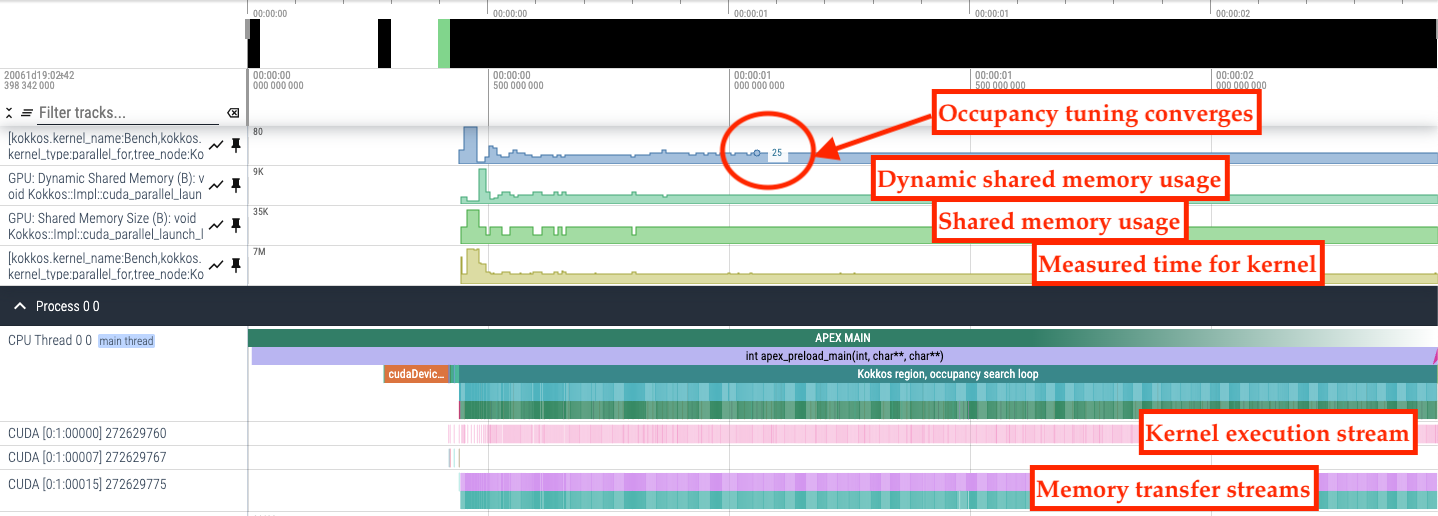
\includegraphics[width=\linewidth]{4_5/tuning/nelder_mead_occupancy_trace.png}
    \end{center}
\end{frame}

\begin{frame}[fragile]{Kokkos Potential Future Tuning Plans (7/7)}
  \begin{itemize}
      \item Simplified/abstracted API for custom tuning in user code (or at least some helper functions)
      \begin{itemize}
        \item \texttt{kokkosp\_declare\_[input,output]\_type} - make it easier to create variables
        \item \texttt{kokkosp\_[begin,end]\_context}
        \item \texttt{kokkosp\_request\_values}
      \end{itemize}
      \item Additional examples, performance studies
      \item Internal tuning for \texttt{RangePolicy}
      \item Internal support/testing for more execution engines (SYCL, OpenMP, OpenMPTarget)
  \end{itemize}
\end{frame}

%==========================================================================

%==========================================================================

\begin{frame}[fragile]

  {\Huge Build Systems Updates}

  \vspace{10pt}

\end{frame}

%==========================================================================

% Examples

% note: always keep the [fragile] for your frames!

\begin{frame}[fragile]{New build system features}
  \begin{itemize}
    \item Add support for Zen 4 AMD microarchitecture (\texttt{Kokkos\_ARCH\_ZEN4})
    \item Enable NVIDIA Grace architecture with NVHPC (\texttt{Kokkos\_ARCH\_ARMV9\_GRACE})
    \item Support static library builds via \texttt{CMAKE\_CUDA\_RUNTIME\_LIBRARY=static} when using CUDA as CMake language
  \end{itemize}

\end{frame}

%==========================================================================


%==========================================================================

%==========================================================================

\begin{frame}[fragile]

  {\Huge Deprecations and other breaking changes}

  \vspace{10pt}

\end{frame}


\begin{frame}[fragile]{Intel Classic Compiler}
  \begin{itemize}
    \item Intel has long since deprecated Intel Classic (since around 2022), and removed from oneAPI 2024.0 release
    \item In order to focus on newer compilers, and reduce maintenance burden, we have \textbf{removed} support for Intel Classic (oneAPI Intel/icpx still supported of course!)
  \end{itemize}
\end{frame}


\begin{frame}[fragile]{DualView changes}
  \textbf{Deprecate} direct access to \texttt{d\_view} and \texttt{h\_view}
  \begin{itemize}
    \item Modifying the allocations in d\_view and h\_view directly is dangerous, especially if \texttt{modify} and \texttt{sync} are skipped
    \item Use \texttt{view\_host()} and \texttt{view\_device()} instead
    \item These two functions return by value with deprecated code enabled and by const reference otherwise. This might have perfomance implications if used extensively, e.g., in loop bounds.
  \end{itemize}
\end{frame}


\begin{frame}[fragile]{Experimental SIMD changes}
  \begin{itemize}
    \item \texttt{native\_simd}, \texttt{native\_simd\_mask} \textbf{deprecated} to align with the C++26 standard
    \item \textbf{Removed} Obtaining a reference from \texttt{*simd*::operator[]} to align with the C++26 Standard
    \item \textbf{Changed} the return type of \texttt{Kokkos::Experimental::*simd*::operator==} and \texttt{operator!=} to return SIMD masks instead of \texttt{bool}
    \begin{itemize}
      \item If you want old behavior, use \texttt{all\_of(a == b)}
    \end{itemize}
  \end{itemize}
\end{frame}

\begin{frame}[fragile]{Additional Deprecations and Removals}
  \begin{itemize}
    \item Already discussed deprecating the Makefile
    \item StaticCrsGraph is \textbf{moved} to Kokkos Kernels and \textbf{deprecated} in Core
    \begin{itemize}
      \item See \url{https://github.com/kokkos/kokkos-kernels/pull/2419}
      \item Symbol is in Kernels under \texttt{KokkosSparse::StaticCrsGraph}
    \end{itemize}
  \end{itemize}
\end{frame}
%==========================================================================

% Examples

% note: always keep the [fragile] for your frames!

%\begin{frame}[fragile]{Example list}
%  \begin{itemize}
%      \item Item 1
%      \item Item 2 with some \texttt{code}
%      \begin{itemize}
%        \item Sub-item 2.1
%        \item Sub-item 2.2
%      \end{itemize}
%  \end{itemize}
%\end{frame}

%\begin{frame}[fragile]{Example code}
%    \begin{code}[keywords={std}]
%        #include <iostream>
%        
%        int main() {
%            std::cout << "hello world\n";
%        }
%    \end{code}
%\end{frame}

%\begin{frame}[fragile]{Example table}
%    \begin{center}
%        \begin{tabular}{l|l}
%            a & b \\\hline
%            c & d
%        \end{tabular}
%    \end{center}
%\end{frame}

%==========================================================================


%==========================================================================

\begin{frame}[fragile]{Deprecations}
\begin{itemize}
\item Deprecated \texttt{Kokkos::vector}
\item Use \texttt{std::aligned\_alloc} for all host allocations
\begin{itemize}
\item Removed code that performed allocations with other mechanisms
\item Deprecated \texttt{PosixMemAlign}, \texttt{PosixMMap},
      \texttt{IntelMMAlloc} enumerators from
      \texttt{RawMemoryAllocationFailure::AllocationMechanism}
      which is defined in \texttt{Kokkos::Experimental::}
\item Deprecated the \texttt{HostSpace::AllocationMechanism} enumeration and
      the \texttt{HostSpace(AllocationMechanism)} explicit constructor
\end{itemize}
\end{itemize}
\end{frame}


%==========================================================================

\begin{frame}[fragile]

  {\Huge Bug Fixes}

  \vspace{10pt}

\end{frame}

%==========================================================================

% Examples

% note: always keep the [fragile] for your frames!

%\begin{frame}[fragile]{Example list}
%  \begin{itemize}
%      \item Item 1
%      \item Item 2 with some \texttt{code}
%      \begin{itemize}
%        \item Sub-item 2.1
%        \item Sub-item 2.2
%      \end{itemize}
%  \end{itemize}
%\end{frame}

%\begin{frame}[fragile]{Example code}
%    \begin{code}[keywords={std}]
%        #include <iostream>
%        
%        int main() {
%            std::cout << "hello world\n";
%        }
%    \end{code}
%\end{frame}

%\begin{frame}[fragile]{Example table}
%    \begin{center}
%        \begin{tabular}{l|l}
%            a & b \\\hline
%            c & d
%        \end{tabular}
%    \end{center}
%\end{frame}

%==========================================================================


%==========================================================================


%==========================================================================

\begin{frame}[fragile]

  \vspace{10pt}

  \textbf{How to Get Your Fixes and Features into Kokkos}
  \newline
  \begin{itemize}
    \item Fork the Kokkos repo (\url{https://github.com/kokkos/kokkos})
    \item Make topic branch from \textit{develop} for your code
    \item Add tests for your code
    \item Create a Pull Request (PR) on the main project \textit{develop}
    \item Update the documentation (\url{https://github.com/kokkos/kokkos-core-wiki}) if your code changes the API
    \item Get in touch if you have any question (\url{https://kokkosteam.slack.com})
  \end{itemize}

\end{frame}

%==========================================================================

\end{document}
